\section{Data integrity}

Malleability refers to the ability to make alterations to the ciphertext, without knowledge of the encryption key, resulting in predictable modifications to the plaintext.
This characteristic can be exploited in various ways to launch decryption attacks and manipulate encrypted data.
However, malleability can also be leveraged as a desirable feature, as seen in homomorphic encryption schemes.

To mitigate malleability, it is crucial to design encryption schemes that are inherently non-malleable and incorporate mechanisms to ensure data integrity against attackers. 
While current encryption schemes primarily provide confidentiality, they do not detect changes in the ciphertext effectively.

To address this limitation, a small piece of information known as a tag can be added to the encrypted message, allowing for integrity testing of the encrypted data itself.
Simply adding the tag to the plaintext before encryption is not sufficient, as Message Authentication Codes (MACs) are required for proper data authentication.

\subsection{Message authentication codes}
A message authentication code consists of a pair of functions:
\begin{itemize}
    \item \texttt{compute\_tag(string, key)}: generates the tag for the input string.
    \item \texttt{verify\_tag(string, tag, key)}: verifies the authenticity of the tag for the input string.
\end{itemize}
In an ideal attacker model, the attacker may possess knowledge of numerous message-tag pairs but should be unable to forge a valid tag for a message they do not already know. 
Additionally, tag splicing from valid messages should also be prevented.

\paragraph*{CBC-MAC}
Cipher block chaining message authentication code (CBC-MAC) is a method for generating a fixed-size authentication tag from variable-length messages using a block cipher in CBC mode.
Here's how CBC-MAC works:
\begin{enumerate}
    \item \textit{Initialization}: CBC-MAC operates on fixed-size blocks of data, so if the message is not a multiple of the block size, padding is applied to make it fit. 
        The MAC is initialized with a zero or an initial value.
    \item \textit{Block Encryption}: the message is divided into blocks of equal size. 
        Each block is encrypted using the block cipher in CBC mode. 
        The ciphertext of each block is then XORed with the next plaintext block before encrypting the next block.
    \item \textit{Finalization}: once all blocks are encrypted, the last ciphertext block becomes the MAC.
\end{enumerate}
CBC-MAC possesses several noteworthy characteristics. 
It is computationally efficient, requiring only a single pass through the message. 
The MAC generates a fixed-length authentication tag determined by the block size of the underlying block cipher. 
Additionally, CBC-MAC offers collision resistance, making it extremely difficult to find two different messages that produce the same MAC.
\begin{figure}[H]
    \centering
    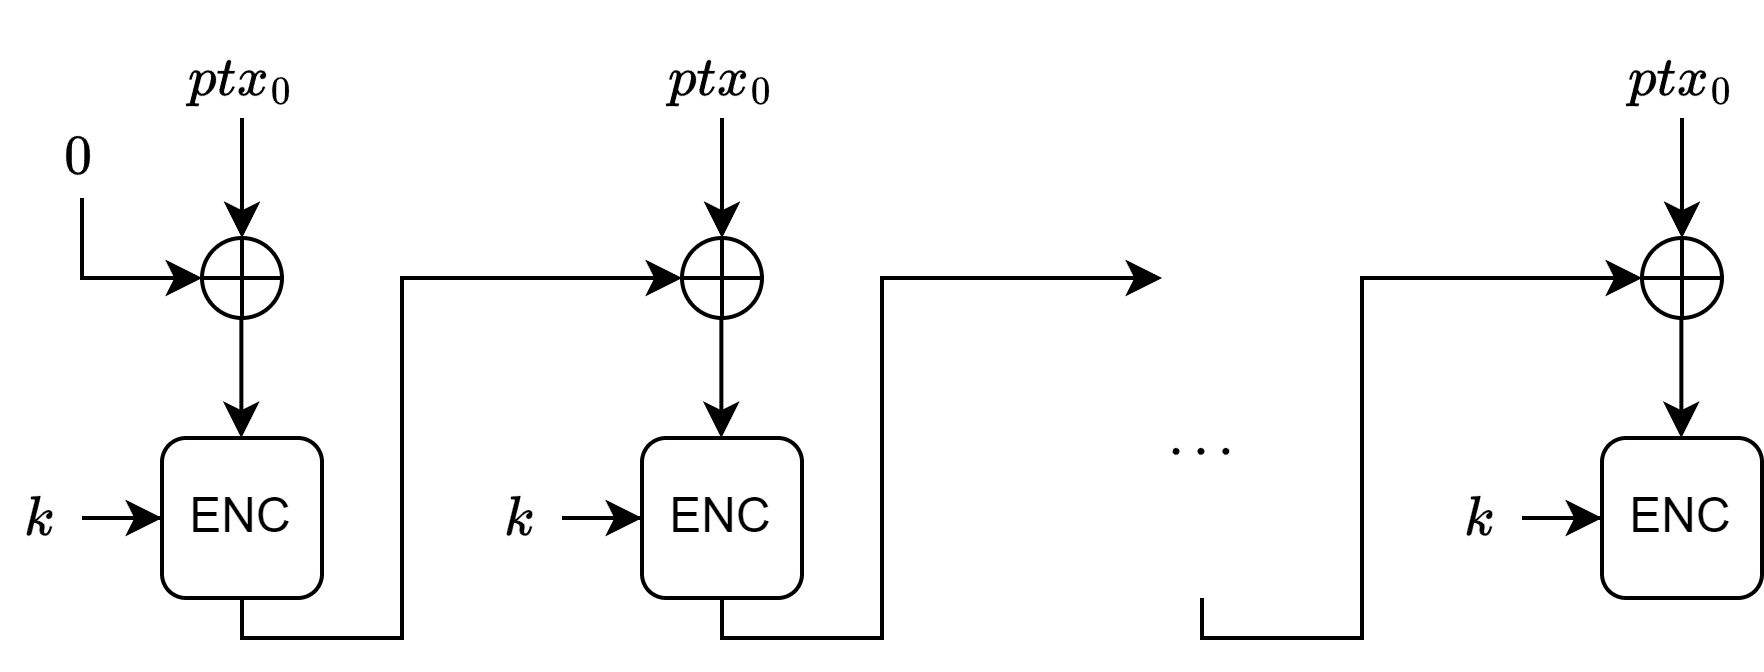
\includegraphics[width=0.75\linewidth]{images/cbcmac.png}
    \caption{CBC encryption mode}
\end{figure}
CBC-MAC is widely used in practice for message authentication in various cryptographic protocols and applications, including network protocols, file authentication, and secure messaging systems. 
However, it is important to use CBC-MAC correctly and securely to avoid potential vulnerabilities.

\paragraph*{MAC usages}
HTTP cookies serve as a form of note to self for HTTP servers, providing a means to store information locally within a user's browser. 
However, it is crucial that this information remains unaltered between server reads. 
To address this concern, the server employs a process where it computes a tag for the cookie using a cryptographic function, denoted as \texttt{compute\_tag(cookie, k)}. 
This tag is then stored alongside the corresponding cookie as a pair (cookie, tag), ensuring the integrity and authenticity of the cookie's contents.

\subsection{Cryptographic hashes}
Ensuring the integrity of a file typically involves either comparing it bit by bit with an intact copy or reading the entire file to compute a message authentication code.
However, it would be highly advantageous to verify the integrity of a file using only short, fixed-length strings, regardless of the file's size, thereby simplifying the process and reducing computational overhead.
Unfortunately, a significant obstacle arises due to the inherent lower bound on the number of bits required to accurately encode a given content without any loss of information. 
This limitation presents a challenge when attempting to devise a method for efficiently testing the integrity of files.

A cryptographic hash function, denoted as $H : \{0, 1\}^\ast \rightarrow \{0, 1\}^I$, is designed such that the following computational problems are difficult to solve:
\begin{enumerate}
    \item Given a digest $d = H(s)$, determining the original input $s$ (first preimage).
    \item Given both an input $s$ and its corresponding digest $d = H(s)$, finding another input $r$ (where $r \neq s$) that produces the same digest ($H(r) = d$) (second preimage).
    \item Finding two distinct inputs $r$ and $s$ (where $r \neq s$) that yield the same digest ($H(r) = H(s)$) (collision).
\end{enumerate}
In an ideal scenario, the performance of a concrete cryptographic hash function can be summarized as follows:
\begin{enumerate}
    \item Finding the first preimage requires approximately $O(2^d)$ hash computations, involving guessing potential inputs $s$.
    \item Finding the second preimage similarly demands around $O(2^d)$ hash computations, involving guessing potential inputs $r$.
    \item Discovering a collision involves approximately $O(2^{2d})$ hash computations.
\end{enumerate}
The resulting output bitstring of a hash function is commonly referred to as a digest.

\paragraph*{Hash functions}
For preferred cryptographic hash functions, consider utilizing SHA-2 and SHA-3. 
SHA-2, developed privately by the NSA, offers digest sizes of 256, 384, and 512 bits. 
SHA-3, on the other hand, emerged from a public design contest akin to AES and boasts digest sizes ranging from 256 to 512 bits. 
Both SHA-2 and SHA-3 are currently unbroken and enjoy wide standardization by bodies such as NIST and ISO.

Conversely, it's advisable to steer clear of SHA-1 and MD-5. 
SHA-1, with its fixed 160-bit digest size, has been compromised for collisions, achievable in around $2^{61}$ operations. 
MD-5, which is known to be severely broken, allows for collisions with just $2^{11}$ operations, with public tools readily accessible for generating collisions. 
MD-5 is particularly vulnerable to collisions with arbitrary input prefixes, achievable in approximately $2^{40}$ operations.

\paragraph*{Usage}
Hash functions serve various purposes, including:
\begin{itemize}
    \item \textit{Pseudonymized matching}: employed in scenarios like signal's contact discovery, where hashes of values are stored and compared instead of the actual values themselves.
    \item \textit{MAC construction}: hash functions are integral in generating Message Authentication Codes (MACs), where a tag is produced by hashing both the message and a secret string. 
        Verification involves recomputing the same hash and comparing it with the original tag. 
        HMAC (Hash-based Message Authentication Code) is a widely adopted method, standardized in RFC 2104 and NIST FIPS 198. 
        It utilizes a generic hash function as a plug-in, denoted as HMAC-hash name. 
        Examples include HMAC-SHA1, HMAC-SHA2, and HMAC-SHA3.
    \item \textit{Forensic applications}: hash functions are crucial in forensic investigations. 
        For instance, only the hash of a disk image obtained can be documented in official reports, ensuring data integrity and facilitating verification processes.
\end{itemize}